\section{Overall description}
The purpose of this section is to provide a brief description of the project and to describe known actors and their interaction with the system. The section presents a high level view. For more detailed information, please refer to the developer team.

	\subsection{Stakeholders}
	\begin{itemize}
		\item \textbf{Rowing club administrators:} Must integrate the system into the rowing club's network infrastructure. Their concern is, that the system is usable for logging routes without any extended knowledge of computer systems.
		\item \textbf{Developers:} JEE course students, that are developing the system. Developers include architects, testers and quality engineers.
		\item \textbf{Rowing club members:} Use the system to log their rowed routes.
		\item \textbf{Lecturer:} Checks the state of development and marks the result of the developers for the JEE course.
		\item \textbf{Rowing club:} Organization that profits from the system, because it offers the possibility to create detailed statistics and provides a log.
		\item \textbf{Insurance company:} Interested in accident cases to view logged routes.
	\end{itemize}
	
	\subsection{Actors}
	The following actors can be defined:\\
	
	\begin{itemize}
		\item \textbf{Rowing club administrator:} The rowing club administrator uses the system to create and publish boats and routes. Rowing club administrators also use the system to generate analysis and view statistics. Another task of him is to observe the status of boats for retrieving information about damaged boats.
		\item \textbf{Rowing club member:} The rowing club member uses the system to log their rowed routes and publish these routes on their profile.
	\end{itemize}
	
	
	\subsection{Use case Model Survey}
	According to the six parts identified in section \ref{scope}, the use case model is broken into packages. The use cases presented in this survey are high level use cases and are presented in figure \ref{img:rowbuddyPackages}.
	
	\begin{figure}[H]
		\begin{center}
			\includegraphics[width=0.5\textwidth]{./figures/RowBuddy_packages.pdf}
			\caption{RowBuddy Packages}
			\label{img:rowbuddyPackages}
		\end{center}
	\end{figure}

		\subsubsection{Package RowBuddy Boat Management}

		\begin{figure}[H]
			\begin{center}
				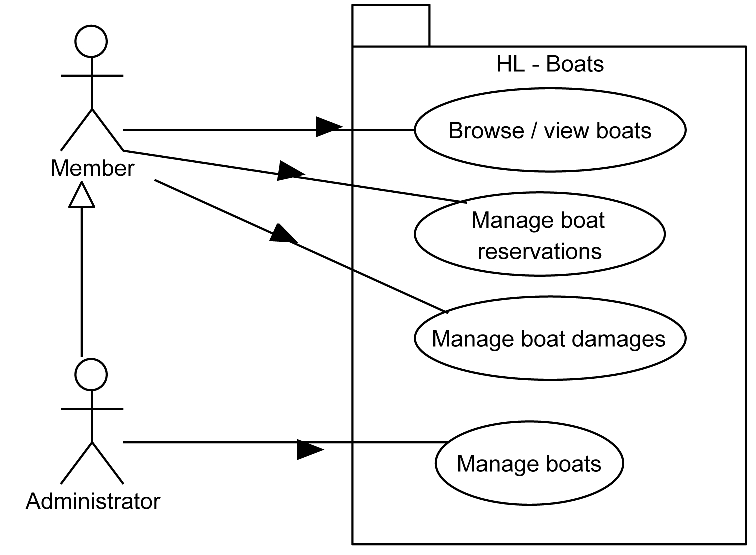
\includegraphics[width=0.6\textwidth]{./figures/HL-BoatManagement.pdf}
				\caption{Use case diagram package boat management}
				\label{img:UCBoatManagement}
			\end{center}
		\end{figure}

		\hluc{HLUC-1}{Browse / view boats}{Boats}{1}{gef}{}{%
A member can browse through the boats that exist in the system and view the details of a boat. The detail view of a boat contains information about the properties of a boat like the number of rowers and information about if the boat has a cox.}

		\hluc{HLUC-2}{Manage boats}{Boats}{1}{gef}{}{%
An administrator can add, edit and delete boats in the system. A boat that is deleted is completely removed from the system as long as it is not used in any other part of the system. If it is deleted and still referenced anywhere, it is visible in any parts where it is referenced, but it cannot be selected any longer for boat relevant actions. A boat can be locked and unlocked so that it cannot be used for trips if it is broken or under repair. }

		\hluc{HLUC-3}{Manage boat reservations}{Boats}{1}{gef}{}{%
If a member wants to use certain boats at a certain point in the future he is able to reserve them. Therefore he can select a time period and boats that are available during that time. If boats are blocked by other reservations he is able to see that, too. A reservation can be modified or deleted by the person that has created it and an administrator. Modification includes the adding and removing of additional boats. During reservation time the reserved boats can only be used by the person that has reserved the boat. }

		\hluc{HLUC-4}{Manage boat damages}{Boats}{1}{gef}{}{%
A member can record a damage that has occured on a boat. He browses for a boat and chooses to add a damage. He enters information about the damage on the boat and additional information on the circumstances how the damage has happened. The creator and an administrator is able to edit the damage. An administrator can resolve the damage as fixed. A damage that is not fixed yet does not block a boat for trips. 
}

		\subsubsection{Package RowBuddy Member Management}

		\begin{figure}[H]
			\begin{center}
				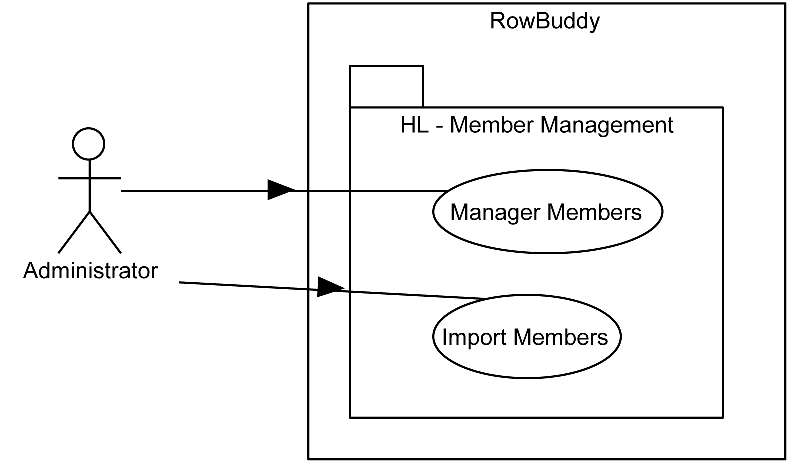
\includegraphics[width=0.6\textwidth]{./figures/HL-MemberManagement.pdf}
				\caption{Use case diagram package member management}
				\label{img:UCMemberManagement}
			\end{center}
		\end{figure}

		\hluc{HLUC-5}{Manage Members}{Member Management}{1}{gef}{}{%
An administrator can manage the members in the system. The information that is stored for a member is his address and the email address. A member can be marked as inaktive. His data is still appearing in all statistical reports. A member can have certain roles. Every member has the role \emph{member}, optionally he can have the role \emph{administrator}. }

		\hluc{HLUC-6}{Import Members}{Member Management}{1}{gef}{}{%
An administrator can import members from a table based file. This is used to import a large amount of member data. A member is identified by its member-id. If a member-id does already exist in the system, all member data is overridden with the imported data.
}
		\subsubsection{Package RowBuddy Member Profiles}

		\begin{figure}[H]
			\begin{center}
				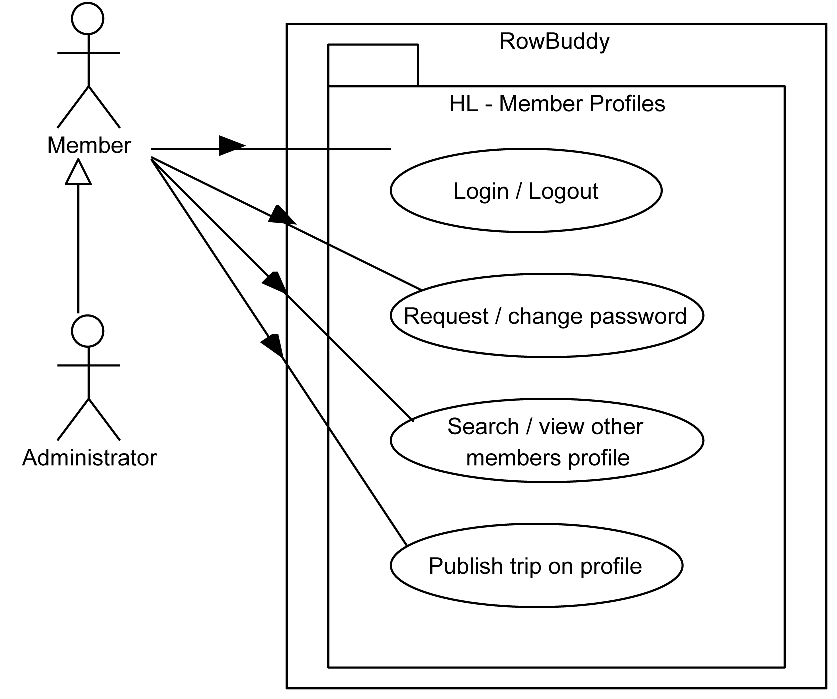
\includegraphics[width=0.6\textwidth]{./figures/HL-MemberProfiles.pdf}
				\caption{Use case diagram package member profiles}
				\label{img:UCMemberProfiles}
			\end{center}
		\end{figure}

		\hluc{HLUC-7}{Login / Logout}{Member Profiles}{1}{gef}{}{%
}

		\hluc{HLUC-8}{Request / change password}{Member Profiles}{1}{gef}{}{%
}

		\hluc{HLUC-9}{Search / view other members profile}{Member Profiles}{1}{gef}{}{%
}

		\hluc{HLUC-10}{Publish trip on profile}{Member Profiles}{1}{gef}{}{%
}

		\subsubsection{Package RowBuddy Route Management}

		\begin{figure}[H]
			\begin{center}
				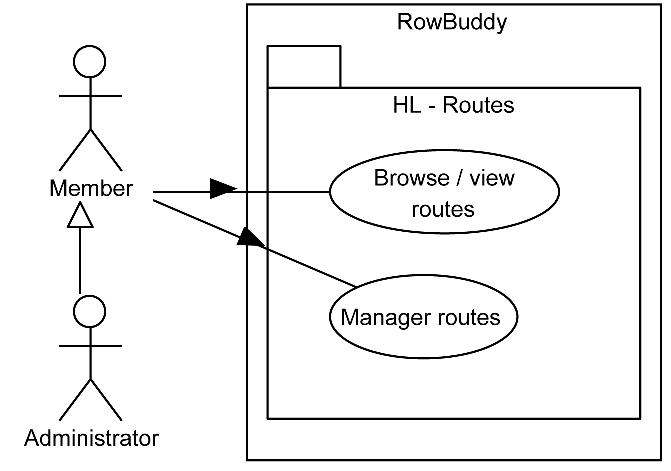
\includegraphics[width=0.6\textwidth]{./figures/HL-Routes.pdf}
				\caption{Use case diagram package routes}
				\label{img:UCRoutes}
			\end{center}
		\end{figure}

		\hluc{HLUC-11}{Browse / view routes}{Routes}{1}{gef}{}{%
A member is able to browse all routes in the system. He can view all details concerning a route. These are a description, the length and a map showing the points of the route. }

		\hluc{HLUC-12}{Manage routes}{Routes}{1}{gef}{}{%
A member can add, edit and delete routes in the system. Routes can be edited and deleted by any member if they are marked as mutable. Otherwise they can only be edited and deleted by the owner and administrators. If a route is modified the trips that have already used this route must not be altered, otherwise the log book would be manipulated. Therefore, edited routes exist as a new version of the route. If the current version of the route is not used yet, no new version has to be created.}

		\subsubsection{Package RowBuddy Statistics}

		\begin{figure}[H]
			\begin{center}
				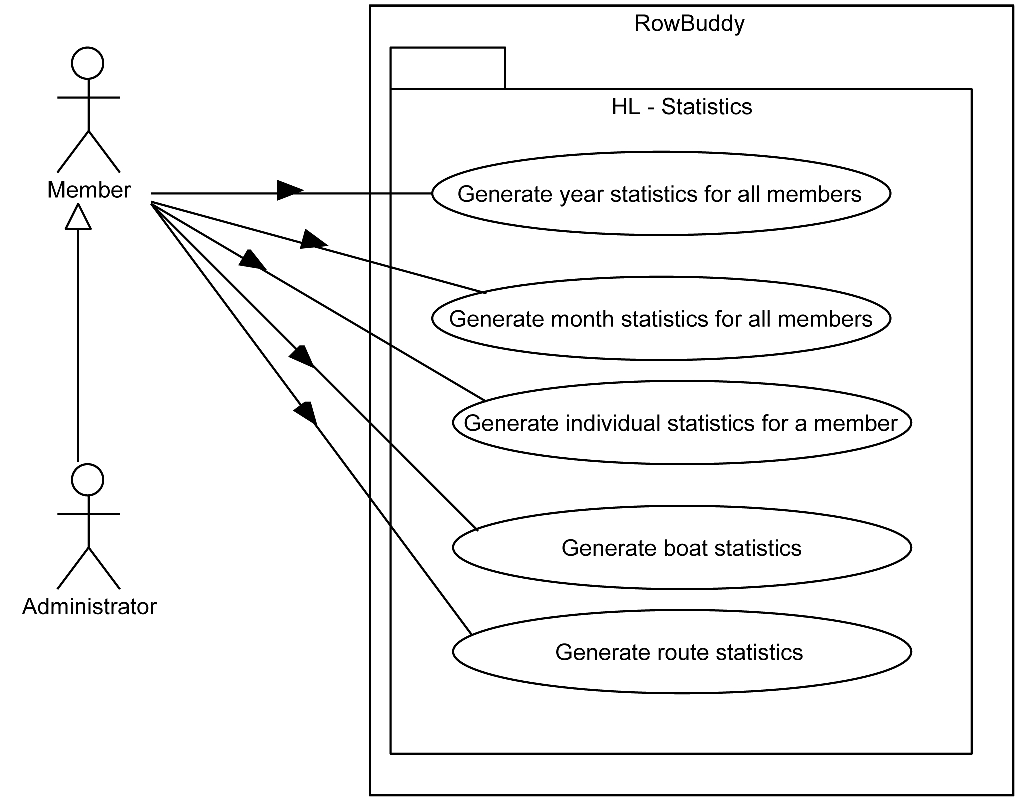
\includegraphics[width=0.6\textwidth]{./figures/HL-Statistics.pdf}
				\caption{Use case diagram package statistics}
				\label{img:UCStatistics}
			\end{center}
		\end{figure}

		\hluc{HLUC-13}{Generate year statistics for all members}{Statistics}{1}{gef}{}{%
}

		\hluc{HLUC-14}{Generate month statistics for all members}{Statistics}{1}{gef}{}{%
}

		\hluc{HLUC-15}{Generate individual statistics fo a member}{Statistics}{1}{gef}{}{%
}

		\hluc{HLUC-16}{Generate boat statistics}{Statistics}{1}{gef}{}{%
}

		\hluc{HLUC-17}{Generate route statistics}{Statistics}{1}{gef}{}{%
}

		\subsubsection{Package RowBuddy Trips}

		\begin{figure}[H]
			\begin{center}
				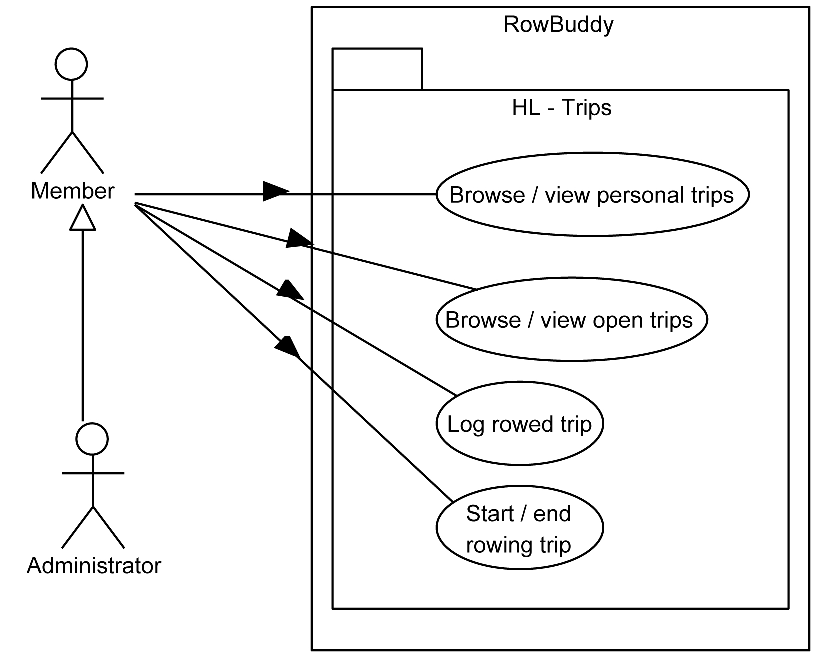
\includegraphics[width=0.6\textwidth]{./figures/HL-Trips.pdf}
				\caption{Use case diagram package trips}
				\label{img:UCTrips}
			\end{center}
		\end{figure}

		\hluc{HLUC-18}{Browse / view personal trips}{Trips}{1}{gef}{}{%
}

		\hluc{HLUC-19}{Browse / view open trips}{Trips}{1}{gef}{}{%
}

		\hluc{HLUC-20}{Log rowed trip}{Trips}{1}{gef}{}{%
}

		\hluc{HLUC-21}{Start / end rowing trip}{Trips}{1}{gef}{}{%
}

\subsection{Domain Model}
The following figure \ref{img:DomainModel} shows the domain model of the RowBuddy system.

		\begin{figure}[H]
			\begin{center}
				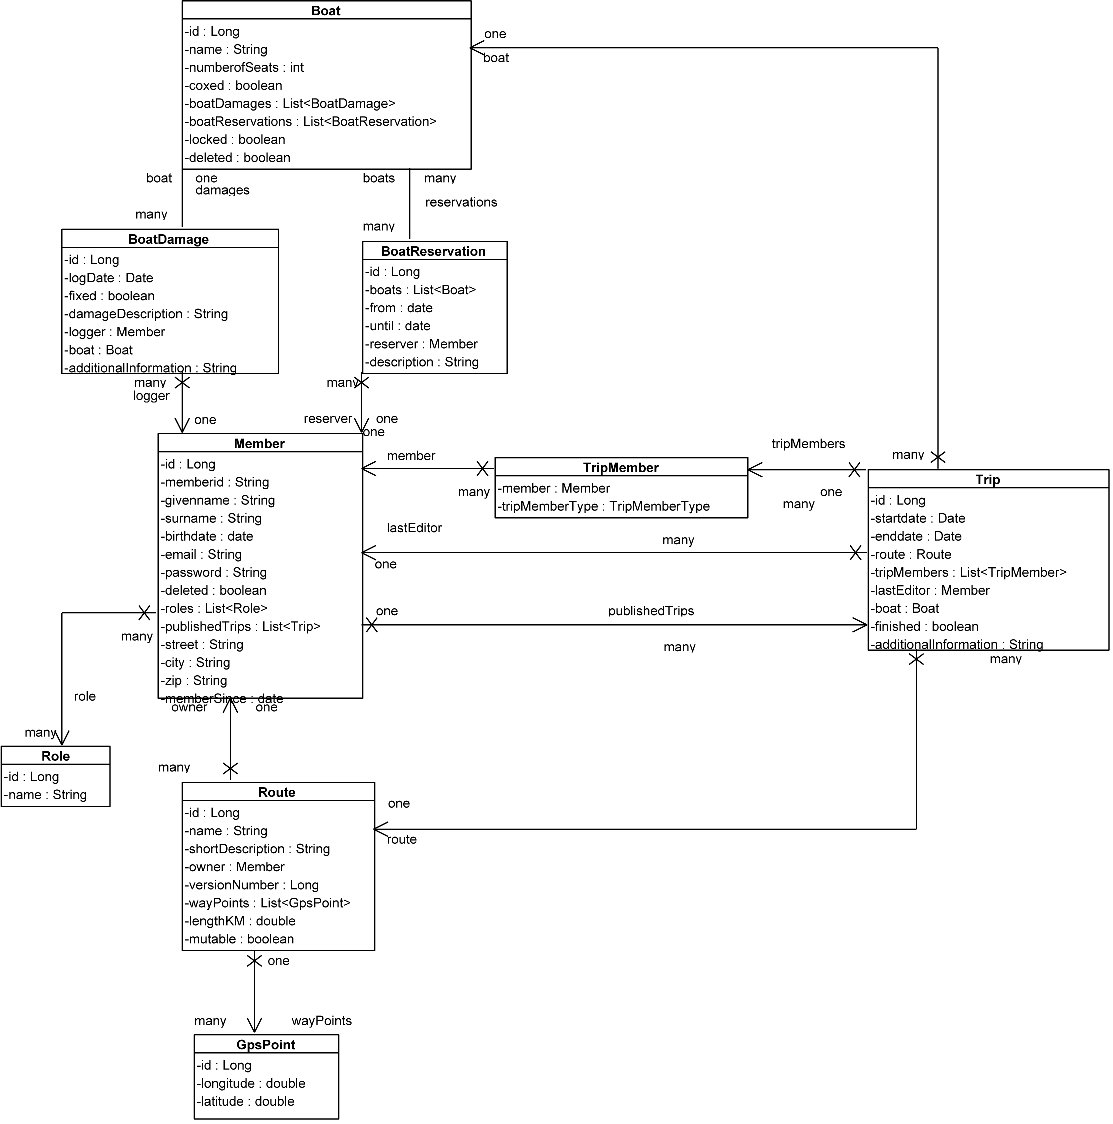
\includegraphics[width=1.0\textwidth]{./figures/DomainModel.pdf}
				\caption{RowBuddy Domain Model}
				\label{img:DomainModel}
			\end{center}
		\end{figure}




		